\section{Lezione del 23 novembre}
Sia $N = (B, E , F)$ una rete elementare, $U \subseteq E$ e $c, c_1, c_2 \subseteq B$. Diciamo che: 
\begin{itemize}
    \item $U$ è un \textbf{insieme di eventi indipendenti }$\iff \forall e_1,e_2 \in U:\ e_1 \neq e_2 \Rightarrow (^\bullet e_1 \cup e_1 ^\bullet) \cap (^\bullet e_2 \cup e_2 ^\bullet) = \emptyset$ 
    \item $U$ è \textbf{un passo abilitato } (insieme di eventi concorrenti) in $c(c[U >)$ se e solo se, $U$ è un insieme di elementi tra loro indipendenti e ogni elemento è abilitato:
    $\forall e \in U:\ c[e>$
    \item $U$ è in \textbf{passo da} $c_1$ a $c_2$, $(c_1[ U > c_2)$ se e solo se l'insieme $U$ è abilitato in $c_1$ e $c_2$ è caso in cui, prendendo $c_1$ togliendo tutt le precondizioni e aggiungendo tutte le post condizioni dell'insieme.\\ $c_1[> U \land c_2 = (c_1 - ^\bullet U) \cup U ^\bullet$
\end{itemize}
{\centering
\begin{tikzpicture}[node distance=2.3cm,>=stealth',bend angle=45,auto]

  \tikzstyle{place}=[circle,thick,draw=blue!75,fill=blue!20,minimum size=6mm]
  \tikzstyle{transition}=[rectangle,thick,draw=blue!75,minimum size=4mm]

    \node [place, tokens=1] (p1)    [label=below:$P_1$]         {}; %P1
    \node [transition] (p) [above left of=p1, label=left:$p$] {}                   %this is new p
        edge [pre ,bend right, blue,thick]  (p1);
    \node [place] (c1) [above right of=p, label=above:$P_2$] {};      %P2
    \node [transition] (p) [above left of=p1] {} %this is new p
        edge [post ,bend left,blue,thick]  (c1);
    \node [transition] (d) [above right of=p1,label=left:$d$] {} %this is d
        edge [pre ,bend right,blue,thick]  (c1)
        edge [post, bend left,blue,thick]  (p1);
        
    \node [place,tokens=1, fill=white,draw=black!75] (b) [right of=d, label=above:$B$] {};
    \node [transition] (d) [above right of=p1] {} %this is d
        edge [post]  (b);
    \node [transition] (e) [right of=b] {} %this is d
        edge [pre]  (b);
    \node[place, tokens=1,fill=red!20,draw=red!75] (c1) [above right of=e, label=above:$C_1$] {};
    \node[place, fill=red!20,draw=red!75] (c2) [below right of=e,label=below:$C_2$ ] {};
    \node [transition,fill=white,draw=red!75] (e) [right of=b,label=right:$e$] {} %this is d
        edge [pre, bend left, red, thick]  (c1)
        edge [post, bend right,red, thick]  (c2);
        
    \node [transition,fill=white,draw=red!75] (c) [above right of=c2,label=right:$c$] {} %this is d
        edge [post, bend right, red, thick]  (c1)
        edge [pre, bend left,red, thick]  (c2);
\end{tikzpicture}
\par}

Da questa figura possiamo capire facilmente le seguenti cose:
\begin{itemize}
    \item $\{p,e\},\{p,c\},\{d,c\}$ sono esempi di insiemi di eventi indipendenti
    \item $\{p,e\}$ è un passo abilitato di $\{P_1,B,C_1\}$
    \item $\{P_1,B,C_1\}[\{p,e\} >\{P_2,C_2\} $
\end{itemize}

Un \textbf{sistema elementare} $\Sigma = (B,E,F, c_{in})$ è definito da una rete $N = (B, E , F)$ e da $c_{in} \subseteq B$ che rappresenta un caso iniziale della rete. \\
L'insieme dei \textbf{casi raggiungibili} ($C_{\Sigma}$) del sistema elementare $\Sigma = (B,E,F, c_{in})$ è il più piccolo sottoinsieme di $2^B$ tale che:
\begin{itemize}
    \item il caso iniziale appartiene all'insieme dei casi raggiungibili: $c_{in} \in C_{\Sigma}$.
    \item se $c$ è un caso raggiungibile, $U$ è un insieme di eventi indipendenti abilitati in $c$,e nel momento in cui $U$ è abilitato in c questo mi porta in $c'$ allora anche $c'$ è raggiungibile: $c \in C_{\Sigma}$ e $U \subseteq E$, $c' \subseteq B$ sono tali che se $c[U > c' \implies c' \in C_{\Sigma}$. 
\end{itemize}
In questo modo ho definiti tutti i casi raggiungibili $C_{\Sigma}$ partendo da $c_{in}$.\\

Possiamo definire, dato un sistema, anche l'insieme dei possibili passi abilitati in un qualche caso raggiungibile. \\ Diremo che $U_{\Sigma}$ è l'insieme dei passi di $\Sigma : \{U \subseteq E \ | \ \exists c,c'\in C_{\Sigma}: \ c[U >c' \}$

\subsection{Il comportamento dei sistemi elementari}
Sia $\Sigma = (B,E,F, c_{in})$ un sistema elementare,  $c_{i} \in C_{\Sigma}$. e  $e_{i} \in E$.
\begin{itemize}
    \item si vanno a considerare tutte le possibili sequenze di eventi partendo dal caso iniziale. Quindi si studia il \textbf{comportamento sequenziale}, riotteniamo la semantica di interleaving (simulazione sequenziale non deterministica), per esempio osserviamo una sequenza ottenuta da un sistema finito, dove quindi non si presentano loop (ci sono due possibili notazioni che possiamo utilizzare):
    $c_{in} [e_1  > c_1[e_2 > \dots [e_n > c_n$ oppure $c_{in} [e_1\ e_2 \dots e_n> c_n$
    \item si possono descrivere anche i comportamenti non sequenziali, descrivendo quindi le sequenze di passi, tenendo conto che $U_i$ rappresentano semplicemente sotto insieme di eventi che sono indipendenti e possono scattare in sequenza:  
    $c_{in} [U_1  > c_1[U_2 > \dots [U_n > c_n$ oppure $c_{in} [U_1\ U_2 \dots U_n> c_n$
    \item in fine abbiamo il comportamento non sequenziale, o processi non sequenziali, che danno origine al \textit{partial order semantics}, andando a considerare l'ordine parziale che esiste tra gli eventi.
\end{itemize}
Si ricorda che si possono utilizzare sequenze sia finite che infinite di passi o eventi. 
{\centering
\begin{tikzpicture}[node distance=1.3cm,>=stealth',bend angle=45,auto]
  \tikzstyle{place}=[circle,thick,draw=blue!75,fill=blue!20,minimum size=6mm]
  \tikzstyle{transition}=[rectangle,thick,draw=blue!75,minimum size=4mm]

    \node [place, tokens=1] (uno)   [label=right:$1$]         {}; %P1
    \node [transition] (a) [below of =uno] {}
        edge [pre]  (uno);
    \node [place ] (tre)[label=right:$3$]  [below of =a]       {}; %P1
    \node [transition] (a) [below of =uno,label=left:$a$] {}
        edge [post]  (tre);
    \node [transition] (c) [right of =a, label=right:$c$] {}
        edge [post]  (uno)
        edge [pre] (tre);
    \node [place, tokens=1] (due)  [above right of = c,label=right:$2$]         {}; %P1
    \node [place]       (quattro)  [below right of = c,label=right:$4$]         {}; %P1    
    \node [transition]        (c)  [right of =a,label=right:$c$] {}
        edge [post]  (due)
        edge [pre] (quattro);
     \node [transition] (b) [right of = c,label=right:$b$] {}
        edge [post]  (quattro)
        edge [pre] (due);
    \node [transition] (d) [below of = tre,label=above:$d$] {}
        edge [pre]  (quattro)
        edge [pre, bend left] (uno);
    \node [place]       (cinque)  [right of = d,label=right:$5$]         {}; %P1    
    \node [transition] (e) [below of = tre,label=above:$d$] {}
        edge [post]  (cinque);
\end{tikzpicture}
\par}

In questo caso abbiamo che una possibile sequenza di occorrenze di eventi è data da:
\begin{itemize}
    \item $\{1,2\}[a> \{3,2\}[b > \{3,4\}[c>\{1,2\}[b> \{1,4\}[d>\{5\}$
\end{itemize}
Invece una possibile sequenza di passi è data da:
\begin{itemize}
    \item $\{1,2\}[\{a,b\} > \{3,4\}[\{c\} > \{1,2\}[\{b\}> \{1,4\}$
\end{itemize}
Invece una processo non sequenziale di $\Sigma$:
\begin{figure}[H]
    \centering
    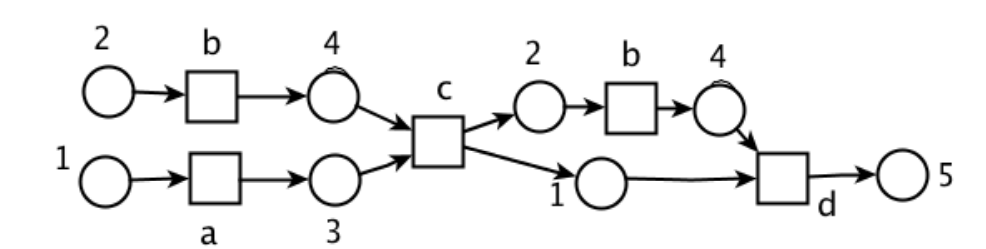
\includegraphics[scale = .5]{IMM/seq_immag_1.PNG}
\end{figure}

\subsection{Grafi dei casi raggiungibili}
Il comportamento di un sistema elementare $\Sigma = (B,E,F, c_{in})$ può essere rappresentato dal suo grafo dei casi. \\
Il \textbf{grafo dei casi} di $\Sigma$ è il sistema di transizioni etichettato $GG_{\Sigma}  = (C_{\Sigma},U_{\Sigma}, A, c_{in})$ dove:
\begin{itemize}
    \item $C_{\Sigma}$ è l'insieme dei nodi del grafo (gli stati globali)
    \item $U_{\Sigma}$ è l’alfabeto
    \item $A$ è l'insieme di archi etichettati 
    \[A = \{(c, U, c')| c, c' \in C_{\Sigma}, U \in U_{\Sigma}, c[U > c' \}\]
    \begin{figure}[H]
        \centering
    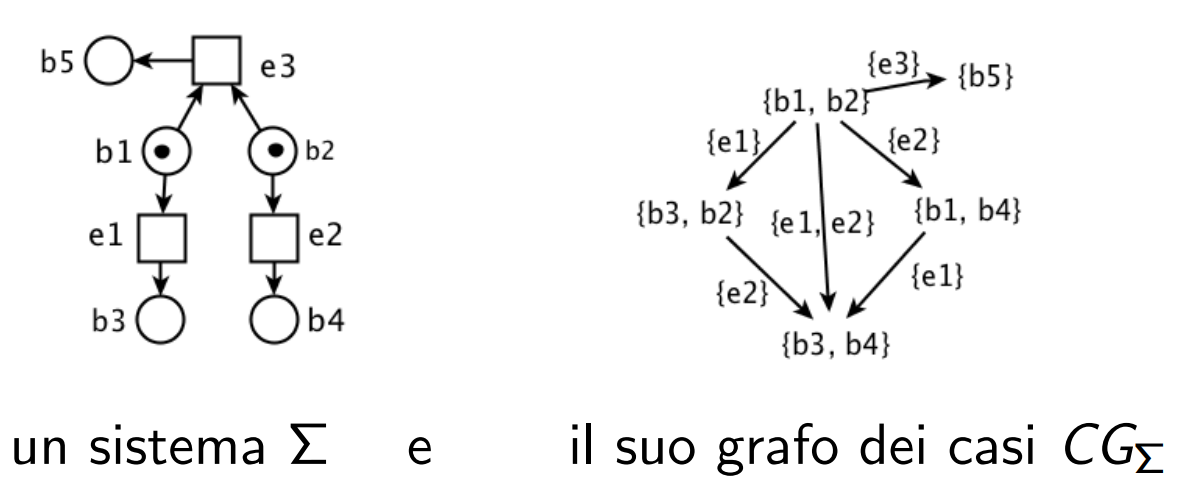
\includegraphics[scale = .5]{IMM/seq_immag_2.PNG}
\end{figure}
\end{itemize}


\subsection{Diamond Property}
Dato un sistema elementare $\Sigma = (B,E,F;c_{in})$ e il suo grafo dei casi $CG_\Sigma=(C_\Sigma, U_\Sigma, A, c_{in})$ si ha che il grafo soddisfa una particolare proprietà, detta \textbf{diamond property}, tipica solo dei sistemi elementari.
La \textbf{diamond property} stabilisce una proprietà della struttura del grafo della rete elementare, ovvero, dati $U_1,U_2\in U_\Sigma$ tali che:$U_1\cap U_2=\emptyset$,$U_1\neq\emptyset$ e  $U_2\neq\emptyset$ e dati $c_i\in C_\Sigma$ allora vale, per esempio:
\begin{figure}[H]
    \centering
    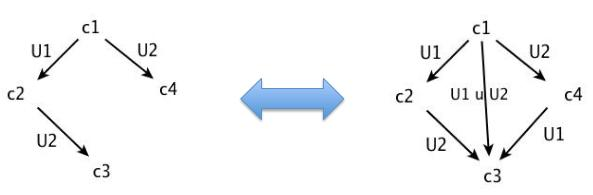
\includegraphics[scale = 0.6]{IMM/diamond.jpg}
    \label{fig:dia}
\end{figure}
ovvero se posso rilevare come sottografo una struttura come quella a sinistra nell'immagine allora sicuramente tale sottografo contiene anche gli archi per ottenere l'immagine di destra. Si possono fare delle prove:
\begin{enumerate}
  \item \textbf{prima prova:}\\
  Dimostriamo che possiamo passare all'immagine di destra da quella di sinistra aggiungendo i due archi mancanti.\\ Diciamo che $U_i$ è un singolo evento $e_i$, con $i=1,2$. Siano inoltre $c_1,c_2\in C_\Sigma$, ovvero sono casi raggiungibili, ed $e_1,e_2\in E$ tali che $c_1 [e_1 > c_2 [e_2 > \mbox{ e } c_1 [e_2 >$. Si vuole dimostrare che: \[(^\bullet e_1\cup e_1^\bullet)\cap(^\bullet e_2\cup e_2^\bullet)=\emptyset\] ovvero che i due eventi sono indipendenti, che sono entrambi abilitati e che sono eseguibili in qualsiasi ordine. 
  Da $c_1 [e_1 > \mbox{ e }c_1 [e_2 >$ segue che:  $^\bullet e_1\cap e_2^\bullet=\emptyset$ e $^\bullet e_2\cap e_1^\bullet=\emptyset$. Infatti se $e_1$ e $e_2$ sono entrambi abilitati in $c_1$, le loro pre-condizioni sono vere e le post-condizioni false, e quindi non è possibile che una condizione sia contemporaneamente precondizione di $e_1$ (vera) e anche postcondizione di $e_2$ (falsa), e viceversa. Quindi le precondizioni di un evento sono disgiunte dalle postcondizioni dell'altro.\\ Inoltre dal fatto che ho $c_1 [e_1 > c_2 [e_2$, ovvero che da $c_1$ è abilitato $e_1$ e che dopo lo scatto di $e_1$ è ancora abilitato $e_2$ possiamo dire che: $e_1^\bullet\cap e_2^\bullet=\emptyset$ e $^\bullet e_1\cap\, ^\bullet e_2=\emptyset$  in $c_2$, infatti, le pre-condizioni di $e_1$ sono false mentre le precondizioni di $e_2$ sono vere e quindi $e_1$ e $e_2$ non possono avere precondizioni in comune; inoltre sempre in $c_2$ le postcondizioni di $e_1$ sono vere, mentre quelle di $e_2$ sono false, e quindi $e_1$ e $e_2$ non possono avere post-condizioni in comune. Quindi le precondizioni dei due eventi sono disgiunte, come del resto anche le postcondizioni, in quanto i due eventi sono sequenziali.\\ Si è quindi dimostrato che i due eventi hanno precondizioni e postcondizioni completamente disgiunte e quindi la tesi è verificata
  \item \textbf{seconda prova:}\\
  Analizzando la situazione:
  \begin{figure}[H]
    \centering
    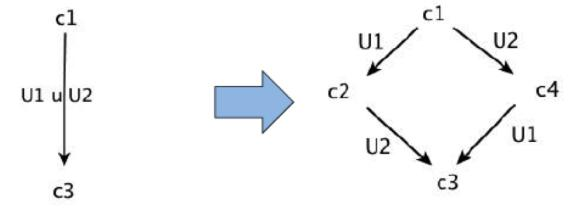
\includegraphics[scale = 0.45]{IMM/diam2.jpg}
  \end{figure}
  Si supponga che $U_1\cup U_2\in U_\Sigma$ e che si abbiano:
  \begin{itemize}
    \item $U_1\cap U_2=\emptyset$, ovvero sono disgiunti
    \item $U_1\neq\emptyset$
    \item $U_2\neq\emptyset$
  \end{itemize}
  allora se $c_1[(U_1\cup U_2)>c_3$, quindi è abilitato il passo $U_1\cup U_2$ in $c_1$, sicuramente si ha che sono abilitati anche i singoli passi:
  \begin{itemize}
    \item $c_1[U_1>$
    \item $c_1[U_2>$
  \end{itemize}
resta da dimostrare che dopo lo scatto di $U_1$ è ancora abilitato $U_2$ in $c_2$. Ma se $U_1\cup U_2$ è un passo abilitato significa che posso eseguirli in qualsiasi ordine, quindi anche prima $U_1$ e poi $U_2$, e questo comporta sicuramente che $U_2$ è abilitato e che porta a $c_3$. Analogamente invertendo $U_1$ e $U_2$, formalmente:
  \begin{itemize}
    \item $c_1[U_1>c_2[U_2>c_3$
    \item $c_1[U_2>c_4[U_1>c_3$
  \end{itemize}
  Si dimostra così che l'immagine di sinistra comporta quella di destra.
\end{enumerate}

\subsection{Grafo dei casi sequenziale}
Un \textbf{grafo dei casi sequenziale} del sistema elementare $\Sigma=(B,E,F;c_{in})$ è una quadrupla in $SCG_\Sigma=(C_\Sigma,E,A,c_{in})$ dove le etichette sono i singoli eventi (mentre il resto rimane definito come nel grafo dei casi raggiungibili). Formalmente si ha quindi che:
$A=\{(c,e,c')|\,c,c'\in C_\Sigma,\,e\in E:\, c[e>c'\}$
\begin{figure}[H]
    \centering
    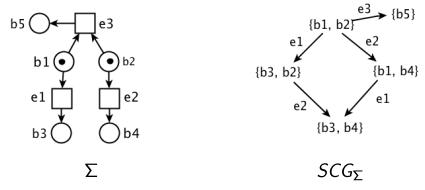
\includegraphics[scale = 0.6]{IMM/seq3.jpg}
\end{figure}
Per la \textbf{diamond property}, nei sistemi elementari il grafo dei casi e il grafo dei casi sequenziale sono \textbf{sintatticamente equivalenti} (possono essere ricavati l’uno dall’altro). Questo implica il fatto che due sistemi elementari hanno grafi dei casi isomorfi se e solo se hanno grafi dei casi sequenziale isomorfi.

\subsection{Isomorfismo tra Sistemi di Transizione Etichettati}
Siano dati due sistemi di transizione etichettati:  $A_1 = (S_1,E_1,T_1,s_{01})$ e $A_2 = (S_2 , E_2 , T_2 , s_{02})$ e siano date due \textbf{mappe biunivoche}:
\begin{enumerate}
    \item $\alpha:S_1\to S_2$, ovvero che passa dagli stati del primo sistema a quelli del secondo
    \item $\beta:E_1\to E_2$, ovvero che passa dagli eventi del primo sistema a quelli del secondo
\end{enumerate}
  allora: \[\langle \alpha,\beta\rangle:A_1= (S_1 , E_1 , T_1 ,s_{01})\to A_2 = (S_2 ,E_2 , T_2 , s_{02})\] è un \textbf{isomorfismo} sse:
\begin{itemize}
    \item $\alpha(s_{01})=s_{02}$, ovvero l'immagine dello stato iniziale del primo sistema coincide con lo stato iniziale del secondo
    \item $\forall s,s'\in S_1,\forall e\in E_1:\,(s,e,s')\in T_1 \Leftrightarrow (\alpha(s),\beta(e),\alpha(s'))\in T_2$ ovvero per ogni coppia di stati del primo sistema, tra cui esiste un arco etichettato $e$, vale che esiste un arco, etichettato con l'immagine di $e$, nel secondo sistema che va dall'immagine del primo stato (considerato del primo sistema) all'immagine del secondo stato (considerato del secondo sistema), e viceversa
  \end{itemize}
  
Due sistemi $\Sigma_1$ e $\Sigma_2$ sono equivalenti  sse hanno grafi dei casi sequenziali, e quindi di conseguenza anche grafi dei casi, \emph{isomorfi}.\\

\subsection{Il Problema della Sintesi}
Dato un sistema di transizioni etichettato $A=(S,E,T,s_0)$, con: 
\begin{itemize}
  \item $S$ insieme degli stati
  \item $E$ insieme delle etichette, ovvero degli eventi
  \item $T$ insieme delle transizioni
  \item $s_0$ stato iniziale
\end{itemize}
ci si propone di stabilire se esiste un sistema elementare $\Sigma=(B,E,F;c_{in})$, tale che l'insieme degli eventi del sistema corrisponda con l'insieme delle etichette di $A$ e tale che il suo grafo dei casi $SCG_\Sigma$ sia isomorfo ad $A$. In caso affermativo costruire $\Sigma$.\\ 

Il problema è stato risolto mediante la cosiddetta \textbf{teoria delle regioni}. Una \textbf{regione} comunque è un particolare sottoinsiemi di stati, legati tramite una certa condizione. Si può però dire che $A$ dovrà soddisfare la diamond property, in quanto altrimenti non sarebbe un sistema di transizioni che potrebbe corrispondere al comportamento di un sistema elementare.

\subsubsection{Contatto}
Sia $\Sigma = (B,E,F;c_{in})$ un sistema elementare e siano $e\in E$ un evento e $c\in C_\Sigma$ un caso raggiungibile dal caso iniziale. Allora si ha che $(e,c)$ è un \textbf{contatto} sse: \[^\bullet e\subseteq c \wedge e^\bullet \cap c \neq\emptyset\] Ovvero, in termini pratici, siamo nel caso in cui un evento $e$ ha le precondizioni vere, si ha quindi che $^\bullet e\subseteq c$, e l'evento non ha tutte le postcondizioni false, quindi $e^\bullet \cap c \neq\emptyset$, allora si dice che l'evento $e$ è in una situazione di contatto e quindi non può scattare.


{
\begin{figure}[H]
    \centering
    
    \begin{tikzpicture}[node distance=2.3cm,>=stealth',bend angle=45,auto]
    
      \tikzstyle{place}=[circle,thick,draw=blue!75,fill=blue!20,minimum size=6mm]
      \tikzstyle{transition}=[rectangle,thick,draw=blue!75,minimum size=4mm]
    
        \node [place, tokens=1] (p1)    [label=below:\mbox{pronto per produrre}]         {}; %P1
        \node [transition] (p) [above left of=p1, label=left:\mbox{produce}] {}                   %this is new p
            edge [pre ,bend right, blue,thick]  (p1);
        \node [place] (c1) [above right of=p, label=above:\mbox{pronto per depositare}] {};      %P2
        \node [transition] (p) [above left of=p1] {} %this is new p
            edge [post ,bend left,blue,thick]  (c1);
        \node [transition] (d) [above right of=p1,label=left:\mbox{deposita}] {} %this is d
            edge [pre ,bend right,blue,thick]  (c1)
            edge [post, bend left,blue,thick]  (p1);
            
        \node [place, fill=white,draw=black!75] (b) [right of=d, label=above:\mbox{buffer pieno}] {};
        \node [transition] (d) [above right of=p1] {} %this is d
            edge [post]  (b);
        \node [transition] (e) [right of=b] {} %this is d
            edge [pre]  (b);
        \node[place, tokens=1,fill=red!20,draw=red!75] (c1) [above right of=e, label=above:\mbox{pronto per prelevare}] {};
        \node[place, fill=red!20,draw=red!75] (c2) [below right of=e,label=below:\mbox{pronto per consumare}] {};
        \node [transition,fill=white,draw=red!75] (e) [right of=b,label=right:\mbox{estrae}] {} %this is d
            edge [pre, bend left, red, thick]  (c1)
            edge [post, bend right,red, thick]  (c2);
            
        \node [transition,fill=white,draw=red!75] (c) [above right of=c2,label=right:\mbox{consuma}] {} %this is d
            edge [post, bend right, red, thick]  (c1)
            edge [pre, bend left,red, thick]  (c2);
                
    \end{tikzpicture}
\caption{Buffer pieno}
\label{buffer-pieno}
\end{figure}
\par}

Sia $\Sigma = (B,E,F;c_{in})$ un sistema elementare. Si dice che il sistema è \textbf{senza contatti} sse: \[\forall e\in E,\,\forall c\in C_\Sigma\mbox{ si ha che } ^\bullet e\subseteq c\Rightarrow e^\bullet\cap c=\emptyset\] ovvero per ogni evento e per ogni caso raggiungibile dal caso iniziale succede sempre che se le precondizioni sono vere, ovvero $^\bullet e\subseteq c$, allora le postcondizioni sono false, ovvero disgiunte dal caso considerato ($e^\bullet\cap c=\emptyset$)

Il quesito che ci poniamo è se è possibile trasformare un sistema elementare $\Sigma$, con contatti, in uno $\Sigma'$, senza contatti, senza però modificarne il comportamento.\\ 
La risposta a questo quesito è affermativa e la procedura consiste nell'aggiungere a $\Sigma$ il complemento di ogni condizione che crea situazione di contatto, ottenendo così un sistema $\Sigma'$ con grafo dei casi isomorfo a quello di $\Sigma$.\\ 

Per aggiungere il complemento, data la condizione $x$, si aggiunge la condizione $not\,\, x$ che sarà vera tutte le volte che $x$ è falsa e viceversa. Per ottenere questo risultato la nuova condizione avrà come pre-eventi i post-eventi di $x$ e come post-eventi i pre-eventi di $x$. Ovvero connetto la nuova condizione agli stessi eventi di quella vecchia ma con archi orientati in senso opposto. Ovviamente le inizializzazioni delle due condizioni dovranno essere opposte (una vera e l'altra falsa).

Se un sistema è senza contatti, sia $\Sigma = (B,E,F;c_{in})$ un sistema elementare \textbf{senza contatti}. Sapendo che se le precondizioni di un evento sono vere allora sicuramente le postcondizioni di quell'evento sono false in quel caso. Quindi se un sistema elementare $|Sigma$ è senza contatti allora per verificare che un evento $e$ sia abilitato in un caso raggiungibile $c$ è sufficiente verificare che le precondizioni di $e$ siano vere . In maniera formale quindi si ha che: 
\[c[e\mbox{ sse } ^\bullet e\subseteq c,\,\,\mbox{ con } e\in E,c\in C_\Sigma\] 

Avendo queste informazioni posso andare a utilizzare una formula più semplice, nella la figura \ref{buffer-pieno} vista in precedenza aggiungendo la condizione complemento si ottiene:

{
\begin{figure}[H]
    \centering
    \begin{tikzpicture}[node distance=2.3cm,>=stealth',bend angle=45,auto]
    
      \tikzstyle{place}=[circle,thick,draw=blue!75,fill=blue!20,minimum size=6mm]
      \tikzstyle{transition}=[rectangle,thick,draw=blue!75,minimum size=4mm]
    
        \node [place, tokens=1] (p1)    [label=below:\mbox{pronto per produrre}]         {}; %P1
        \node [transition] (p) [above left of=p1, label=left:\mbox{produce}] {}                   %this is new p
            edge [pre ,bend right, blue,thick]  (p1);
        \node [place] (c1) [above right of=p, label=above:\mbox{pronto per depositare}] {};      %P2
        \node [transition] (p) [above left of=p1] {} %this is new p
            edge [post ,bend left,blue,thick]  (c1);
        \node [transition] (d) [above right of=p1,label=left:\mbox{deposita}] {} %this is d
            edge [pre ,bend right,blue,thick]  (c1)
            edge [post, bend left,blue,thick]  (p1);
            
        \node [place, fill=white,draw=black!75] (b) [right of=d, label=above:\mbox{buffer pieno}] {};
        
        \node [transition] (d) [above right of=p1] {} %this is d
            edge [post]  (b);
        \node [transition] (e) [right of=b] {} %this is d
            edge [pre]  (b);
        \node [place,tokens=1, fill=white,draw=black!75] (notb) [above of=b, label=above:\mbox{NOT buffer pieno}] {}
            edge [pre]  (e)
            edge [post]  (d);
        \node[place, tokens=1,fill=red!20,draw=red!75] (c1) [above right of=e, label=above:\mbox{pronto per prelevare}] {};
        \node[place, fill=red!20,draw=red!75] (c2) [below right of=e,label=below:\mbox{pronto per consumare}] {};
        \node [transition,fill=white,draw=red!75] (e) [right of=b,label=right:\mbox{estrae}] {} %this is d
            edge [pre, bend left, red, thick]  (c1)
            edge [post, bend right,red, thick]  (c2);
            
        \node [transition,fill=white,draw=red!75] (c) [above right of=c2,label=right:\mbox{consuma}] {} %this is d
            edge [post, bend right, red, thick]  (c1)
            edge [pre, bend left,red, thick]  (c2);
                
    \end{tikzpicture}
\caption{Complemento di buffer pieno}
\label{buffer-pieno-complemento}
\end{figure}
\par}

\subsection{Sequenza}
Sia $\Sigma = (B,E,F;c_{in})$ un sistema elementare, con $c\in C_\Sigma$ un caso raggiungibile dal caso iniziale e $e_1,e_2\in E$ due eventi.\\ 
Si ha che $e_1$ ed $e_2$ sono \textbf{in sequenza} nel caso raggiungibile $c$ sse: \[c[e_1>\wedge\, \neg c[e_2\wedge c[e_1e_2>\] ovvero in $c$ è abilitato $e_1$ ma non $e_2$ ma, dopo lo scatto di $e_1$, $e_2$ diventa abilitato. Quindi in $c$ è possibile attivare prima $e_1$ e poi $e_2$ in sequenza.\\ 
Si ha quindi una relazione di \textbf{dipendenza causale tra $e_1$ ed $e_2$}, ovvero qualche postcondizione di $e_1$ è precondizione di $e_2$ (che quindi può occorrere solo se precedentemente è occorso $e_1$).